%%%%%%%%%%%%%%%%%%%%%%%%%%%%%%%%%%%%%%%%%%%%%%%%%%%%%%%%%%%%%%%%%%%%%%%%%%%
%
%    phase1-AR.tex  (use only for Archival Research and Theory proposals; use phase1-GO.tex
%                     for General Observer and Snapshot proposals and phase1-DD.tex for GO/DD 
%                     proposals or use phase1-MC.tex for GO/MC rapid response proposals.
%                     
%
%    HUBBLE SPACE TELESCOPE
%    PHASE I ARCHIVAL & THEORETICAL RESEARCH PROPOSAL TEMPLATE 
%    FOR CYCLE 24 (2016)
%
%    Version 1.1, August 12,  2015.
%
%    Guidelines and assistance
%    =========================
%     Cycle 23 Announcement Web Page:
%
%         http://www.stsci.edu/hst/proposing/docs/cycle23announce 
%
%    Please contact the STScI Help Desk if you need assistance with any
%    aspect of proposing for and using HST. Either send e-mail to
%    help@stsci.edu, or call 1-800-544-8125; from outside the United
%    States, call [1] 410-338-1082.
%
%%%%%%%%%%%%%%%%%%%%%%%%%%%%%%%%%%%%%%%%%%%%%%%%%%%%%%%%%%%%%%%%%%%%%%%%%%%

% The template begins here. Please do not modify the font size from 12 point.

\documentclass[12pt]{article}
\usepackage{phase1}

\usepackage{graphicx}
%\usepackage{amssymb}

\usepackage{wrapfig}
\usepackage{setspace}
%\usepackage{subfigure}
\usepackage{subcaption}
\usepackage{mathtools}



\graphicspath{/Users/David/Research_Documents/inclination/git_inclination/pilot_paper_code/pilot_paper/paper_figures2/}

\begin{document}

%   1. SCIENTIFIC JUSTIFICATION
%       (see Section 9.1 of the Call for Proposals)
%
%
\justification          % Do not delete this command.
% Enter your scientific justification here.

%The majority of the baryons in the universe are found in the intergalactic medium (IGM). The properties of this important reservoir of matter are most directly measured via absorption in the spectra of UV-bright background QSOs. The UV initiatives undertaken by the Cosmic Origins Spectrograph on HST have produced a wealth of high resolution and high signal-to-noise spectra that are ideal for a wide variety of IGM studies. However, the identification and measurement of spectral features is a major undertaking, and limits the viability of large-scale studies using archival HST data. We propose to create a legacy data archive of all archival COS sightlines, complete with line identifications and measurements. In addition, we will match nearby ($cz \leq 10,000$ km/s) spectral features with probable associated galaxies using the likelihood method we have developed (French et al. 2016, in prep). This will be the first large, publicly accessible IGM absorber dataset, and will provide a legacy artifact directly in line with the NASA Mission Directive whatever-it's-call-thing.

\indent \indent The majority of the baryons in the universe are found in the intergalactic medium (IGM) (e.g. Danforth $\&$ Shull 2008, Lehner et al. 2007, Cen 2013, Dav\'e et al. 2010). Galaxies reside within large filaments of IGM gas (e.g. Wakker et al. 2015), and both draw new material from it for continuing star formation, as well as eject enriched material back into it via feedback. Studying this complex process observationally is challenging, yet paramount to properly understanding and modeling global galaxy evolution.

The properties of this important reservoir of matter are most directly measured via absorption in the spectra of UV-bright background QSOs. Studies using this method have found numerous IGM-galaxy proximity effects, such as increasing absorption equivalent width (CITE), linewidth (e.g. Wakker $\&$ Savage 2009), column density (e.g. Rudie et al 2012), and metallicity (e.g. Kacprzak et al YEAR?) anti-correlating with the distance to the nearest bright galaxy. 

Nevertheless, many open questions remain concerning the details of how gas near to galaxies (the circumgalactic medium or CGM, generally considered to extend to $\sim 2R_{vir}$) interacts with and effects the evolution of the galaxies. Some key questions we would like to answer are:
a) how do the properties of CGM absorbers (e.g. equivalent width, location, velocity) compare to the properties of the galaxies they are associated with (e.g. size, inclination, morphology)?
b) does the CGM follow the rotation direction and velocity of the associated galaxies as predicted by simulations (e.g. Stewart et al. 2011)?

%In order to move forward from these results however, we need to confront several shortcomings that are nearly universal among studies of the IGM-galaxy connection. \\

Previous studies have suffered from several shortcomings in trying to address these questions. We propose a program to deal with these 3 issues in particular:

1) \textbf{\underline{Sample size}}: Probing the CGM in absorption requires a serendipitously located background source, which means that a particular galaxy halo generally only can be probed once. To learn global CGM properties, it is thus necessary to study the statistics of a large dataset of single galaxy-absorber matches. This has not yet been down however, with the largest current CGM surveys maxing out at fewer than 100 galaxy-absorber pairs (e.g. HOW MANY IN A FEW DIFFERENT SURVEYS?).\\


2) \textbf{\underline{Reproducibility}}: In order to correlate CGM absorber properties with a galaxy, a match must be made between a galaxy to an absorption feature, but it is often unclear or arbitrary how this matching is done. Some (e.g. CITATION) simply picked the closest neighboring galaxy to the detected IGM absorber, while others (e.g. CITATION) try to take galaxy size and other properties into account as well. However, different authors continue to use different, subjective criteria, and tend to deal with ambiguities in an ad-hoc manner.\\

3) \textbf{\underline{Incompleteness}}: the completeness of known galaxies decreases sharply with redshift, which can further complicate determining with which galaxy to associated absorption. For example, Mathes et al. (2014) and Werk et al. (2014) are only complete to $\sim L^{\**}$ (at $0.12 < z < 0.67$ and $z\sim0.2$, respectively). Additionally, very few galaxies have published rotation curves, so comparing the velocity of the gas in the CGM to that within the disks of the associated galaxies is usually not possible. Aside from general incompleteness, distant galaxies also tend not to have a classification beyond "massive" or "low-mass". \\

We propose to complete a large scale program to address these issues by using archival COS sightlines to target nearby galaxy-absorber systems. The following sections will discuss in detail how our proposed program address each of the above issues.\\


\noindent \textbf{\underline{1. Increasing the sample size}}\\

\textbf{Archival data:} At the time of writing 550 QSO targets have been observed by COS and are publicly available on MAST. Of these, 300 spectra have S/N$\geq$10 and $z \geq 0.03$, the minimum to be useful for our purposes (anything $z \leq 0.03$, or $cz \leq 10,000$ km/s, is too close to the galaxy velocities). These break down into 3 redshift bins, with 120 at $0.03\leq z \leq 0.2$, 90 at $0.2\leq z \leq 0.45$ and another 90 at $z > 0.45$. Nearly all of these lie within 500 physical kpc of at least one galaxy in the $cz \leq 10,000$ km/s redshift range. In our pilot study of 35 sightlines (French et al. 2016, in prep), we measured 176 Ly$\alpha$ absorption lines, 42 of which we paired with nearby galaxy. Hence, we predict 300 total spectra should produce over 1500 absorption lines and 360 absorber-galaxy pairings.

\textbf{Line Identification}: The UV initiatives undertaken by the Cosmic Origins Spectrograph on HST have produced a wealth of high resolution and high signal-to-noise spectra that are ideal for a wide variety of IGM studies. However, the identification and measurement of spectral features is a major undertaking, and limits the viability of large-scale studies using archival HST data. To combat this we have developed a pipeline that helps automate the IDing of targets, which will allow us to produce a sample of hundreds of spectra and thousands of absorption lines. 

As the final step of our proposed program, we will create a legacy data archive of identifications and measurements of COS sightlines, complete with probable galaxy associations as well.\\


%In attempt to combat these issues, we have begun a large scale survey of nearby COS sightline-galaxy associations, restricting ourselves to $cz \leq 10,000$ km/s, where we have assembled a galaxy catalog complete to $L^{\**}\sim 0.1$. To address the reproducibility issue, we have developed a probability algorithm to automatically choose which galaxy to associate an absorption line with. 
%
%Finally, we have been awarded priority 1 time on the Southern Africa Large Telescope (SALT) in order to measure the rotation curves of 15+ galaxies that have absorption detected in a sightline within 300 kpc and 400 km/s of the galaxy. This data combined with archival COS sightlines will allow us to finally probe how the kinematics of the CGM compare to that of the gas within the disks of galaxies.


\noindent \textbf{\underline{2. Reproducibility}}\\

\textbf{Likelihood Method:} Studies of the circumgalactic medium, or the IGM-galaxy connection, generally rely on matching absorption measured in the spectra of background QSOs to a nearby foreground galaxy. The methods used for matching a galaxy to an IGM absorber are universally ad-hoc, however, and range from picking the nearest galaxy in physical impact parameter, to some combination of impact parameter, size, and judgement. In French et al. (2016, in prep) we are introducing a reproducible, likelihood-based method to streamline these types of decisions. We define the likelihood as follows:

\begin{equation}
	\mathcal{L} = e^{-(\rho/R_{vir})^2} e^{-(\Delta v / 200)^2},
\end{equation}
where $\rho$ is the physical impact parameter between the sightline and a galaxy, $R_{vir}$ is the galaxy's virial radius, and $\Delta v = v_{galaxy} - v_{absorber}$, the difference in velocity between the galaxy and the absorption line. In order for a galaxy to be deemed ``associated" with an absorption line, we require $\mathcal{L}$ for any potentially associated galaxy be a factor of 5 larger than $\mathcal{L}$ for all other galaxies, and $\mathcal{L} \geq 0.001$. This hard limit translates to an absorber located at $\sim 2 R_{vir}$ and $\sim 350$ km/s in physical and velocity separation, respectively. This edge agrees nicely with observational results of \textbf{EXAMPLES AND REFERENCES}.\\


%\begin{figure}[ht!]
%\centering
%  \subfigure[]{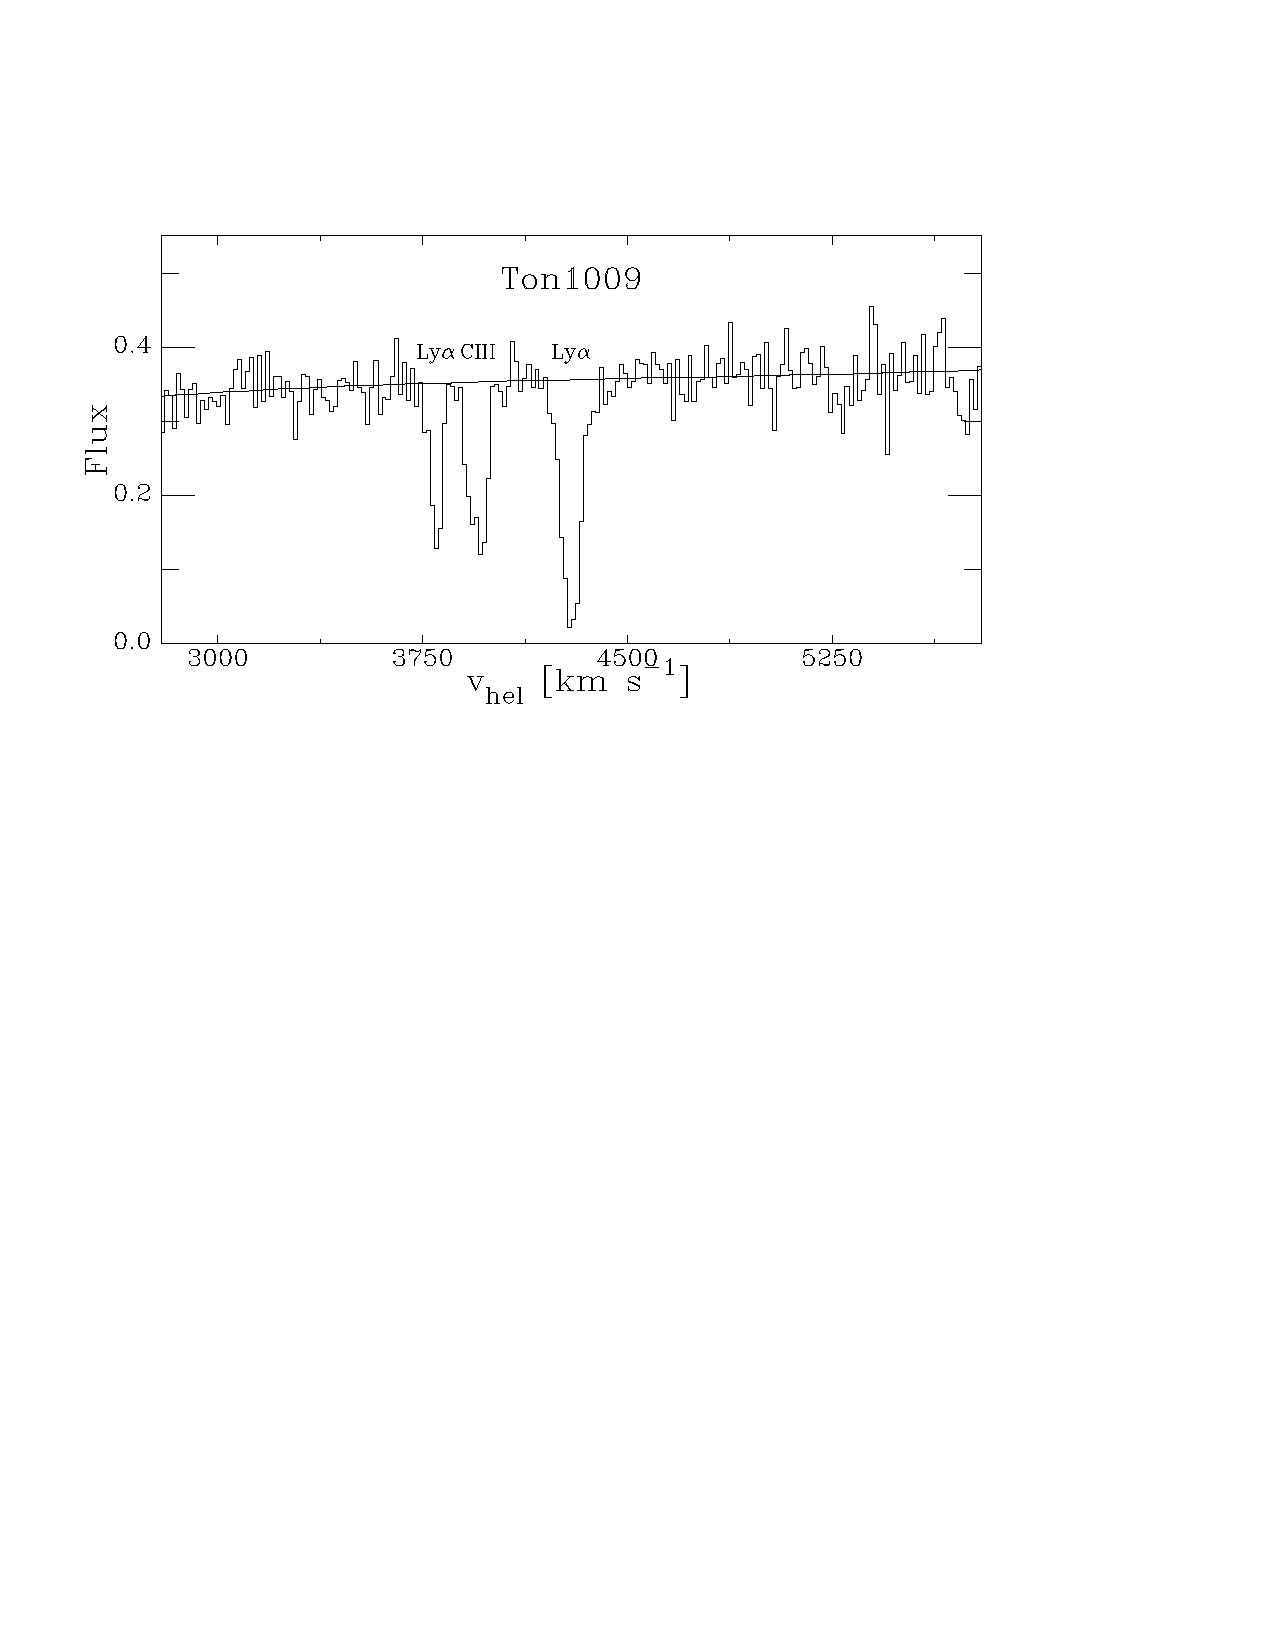
\includegraphics[width=.6\linewidth]{figTON1009_crop.pdf}}{\label{line}}
%  \subfigure[]{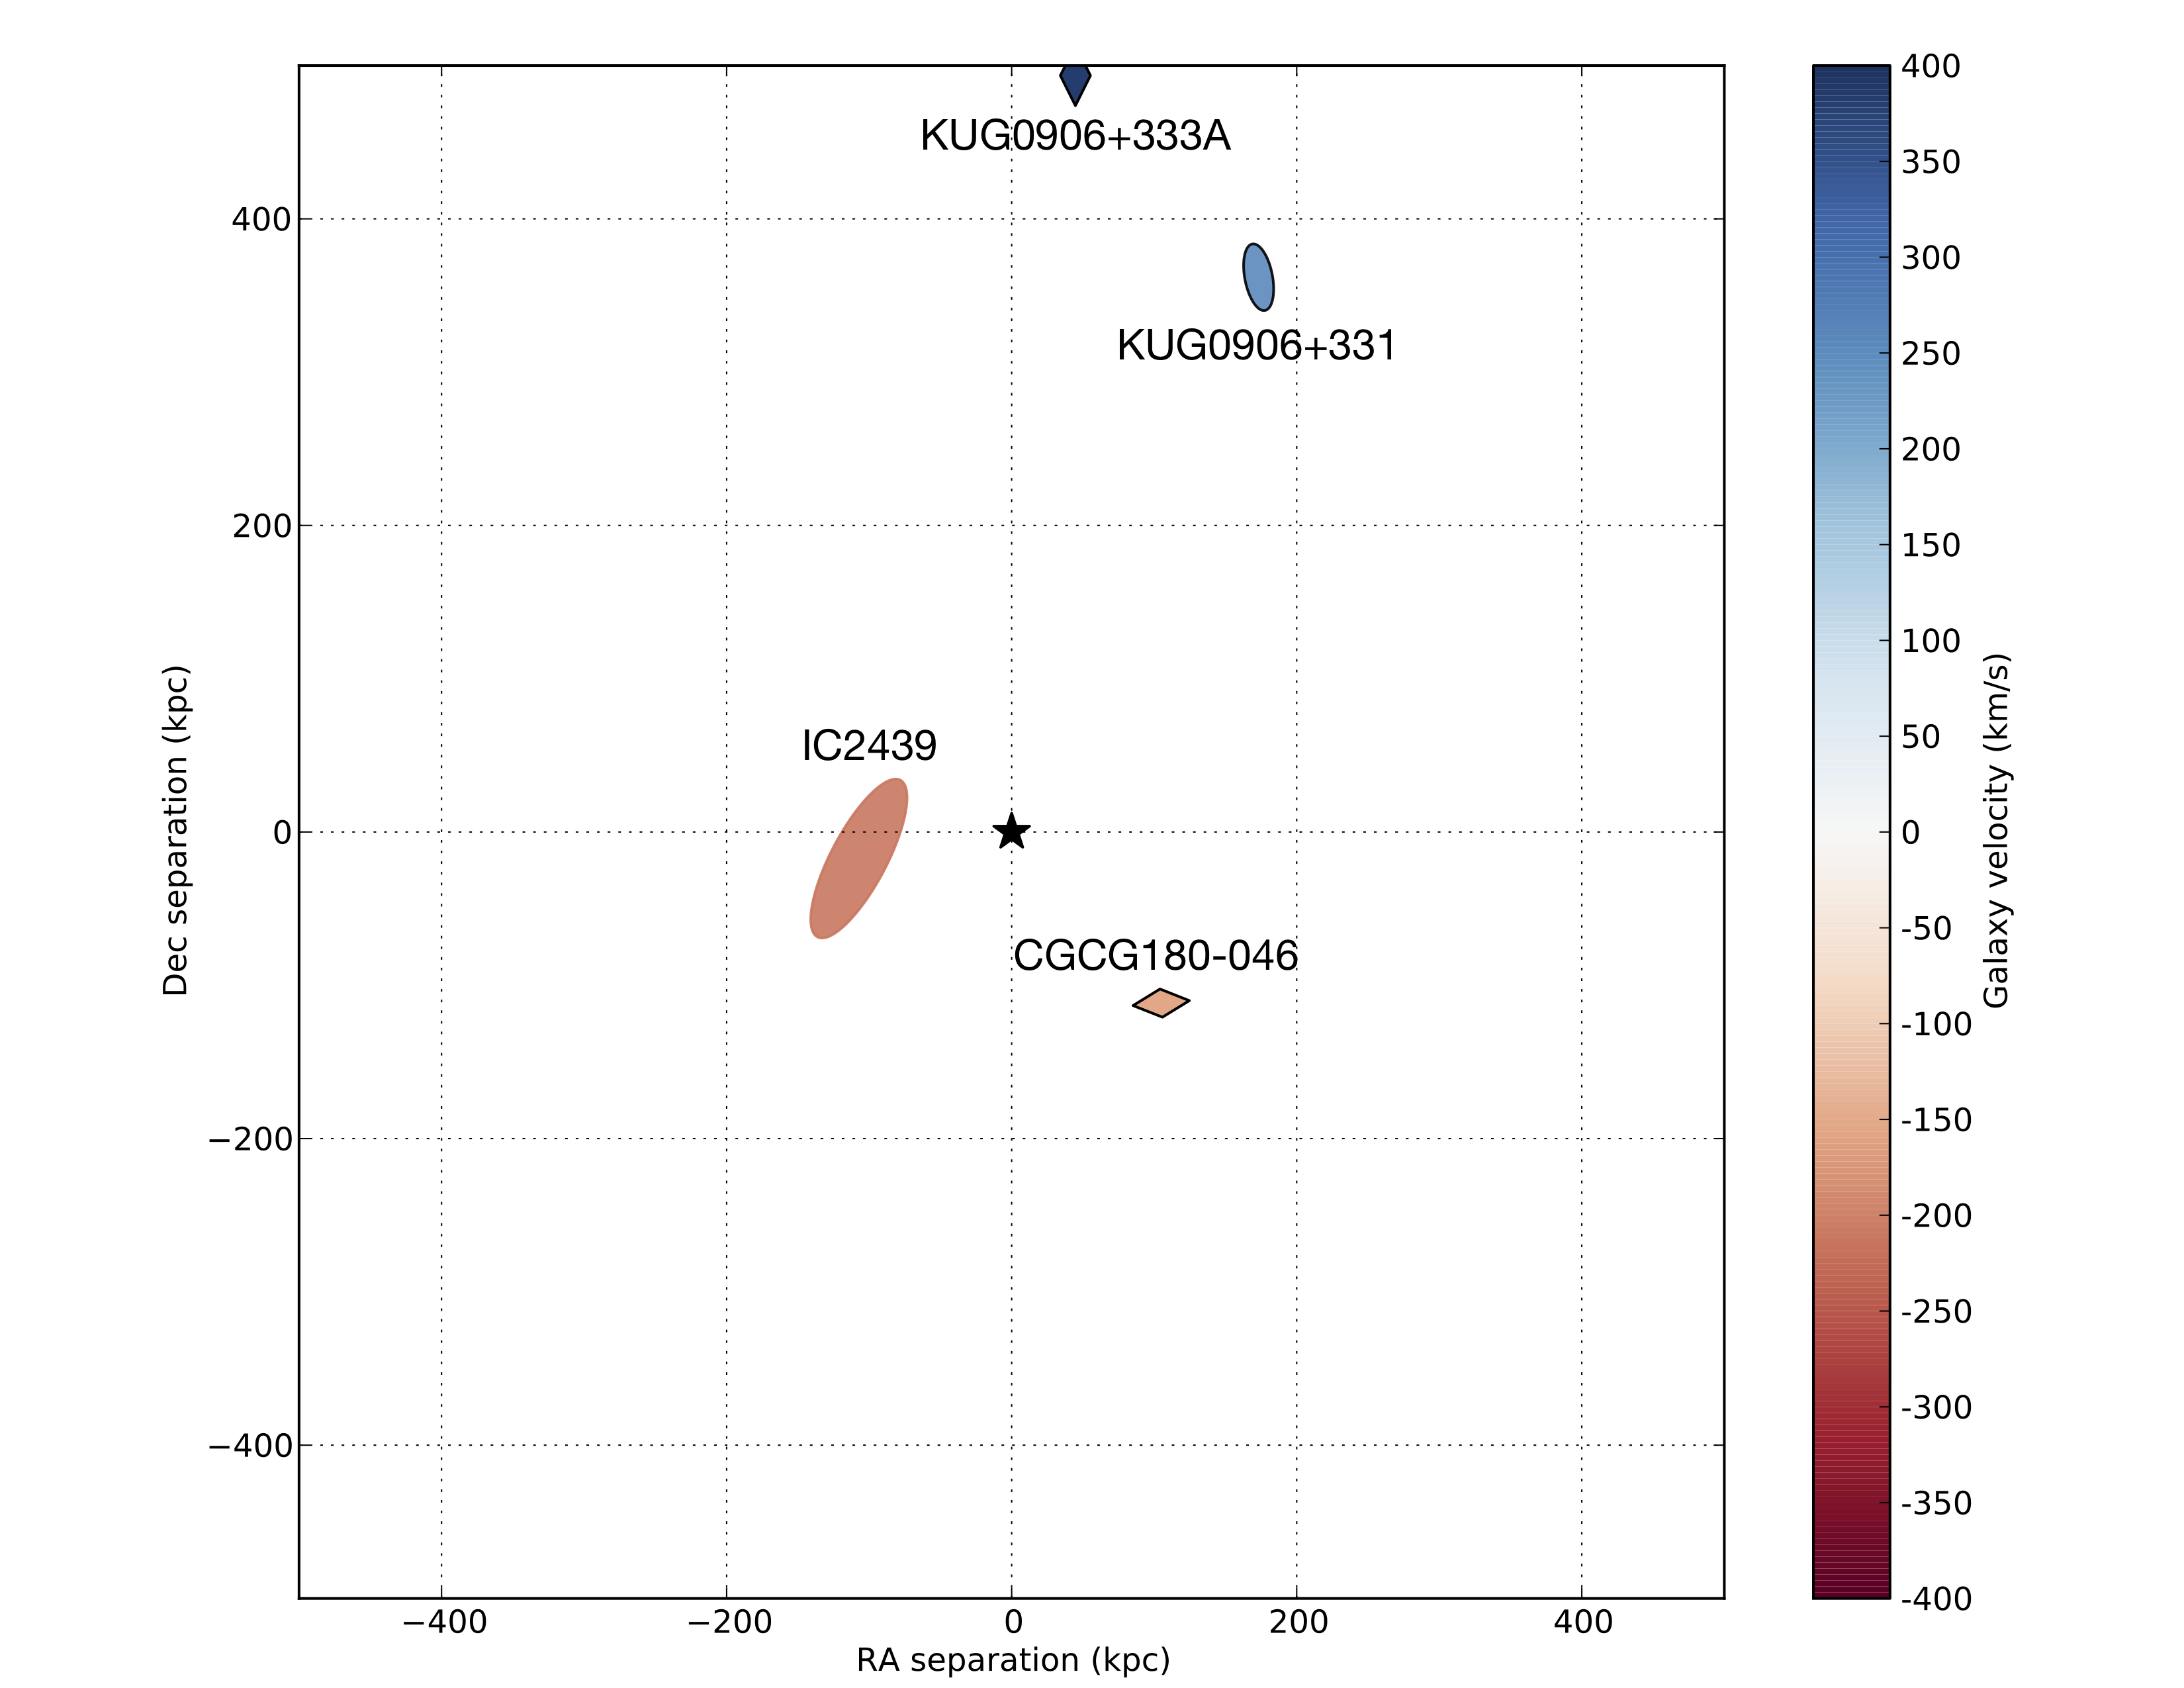
\includegraphics[width=.6\linewidth]{map_TON1009_4285_crop2_labels.png}\label{impactmap}}
%  \caption{\small{a) An example Ly$\alpha$ line found in a sightline towards target TON1009 at 4295 km/s. b) A map of \textit{all} galaxies within a 500 kpc impact parameter target TON1009 sightline and with velocity ($cz$) within 400 km/s of absorption detected at 4295 km/s (central black star). The galaxy IC2439 ($v=4494$ km/s, inclination = $71^{\circ}$) can be unambiguously paired with the Ly$\alpha$ absorption feature at $v=4295$ km/s because it is the largest and closest galaxy in both physical and velocity space to the absorption feature.}}
%\vspace{5pt}
%\end{figure}


\begin{figure}[t!]
    \centering
    \begin{subfigure}[t]{0.5\textwidth}
        \centering
        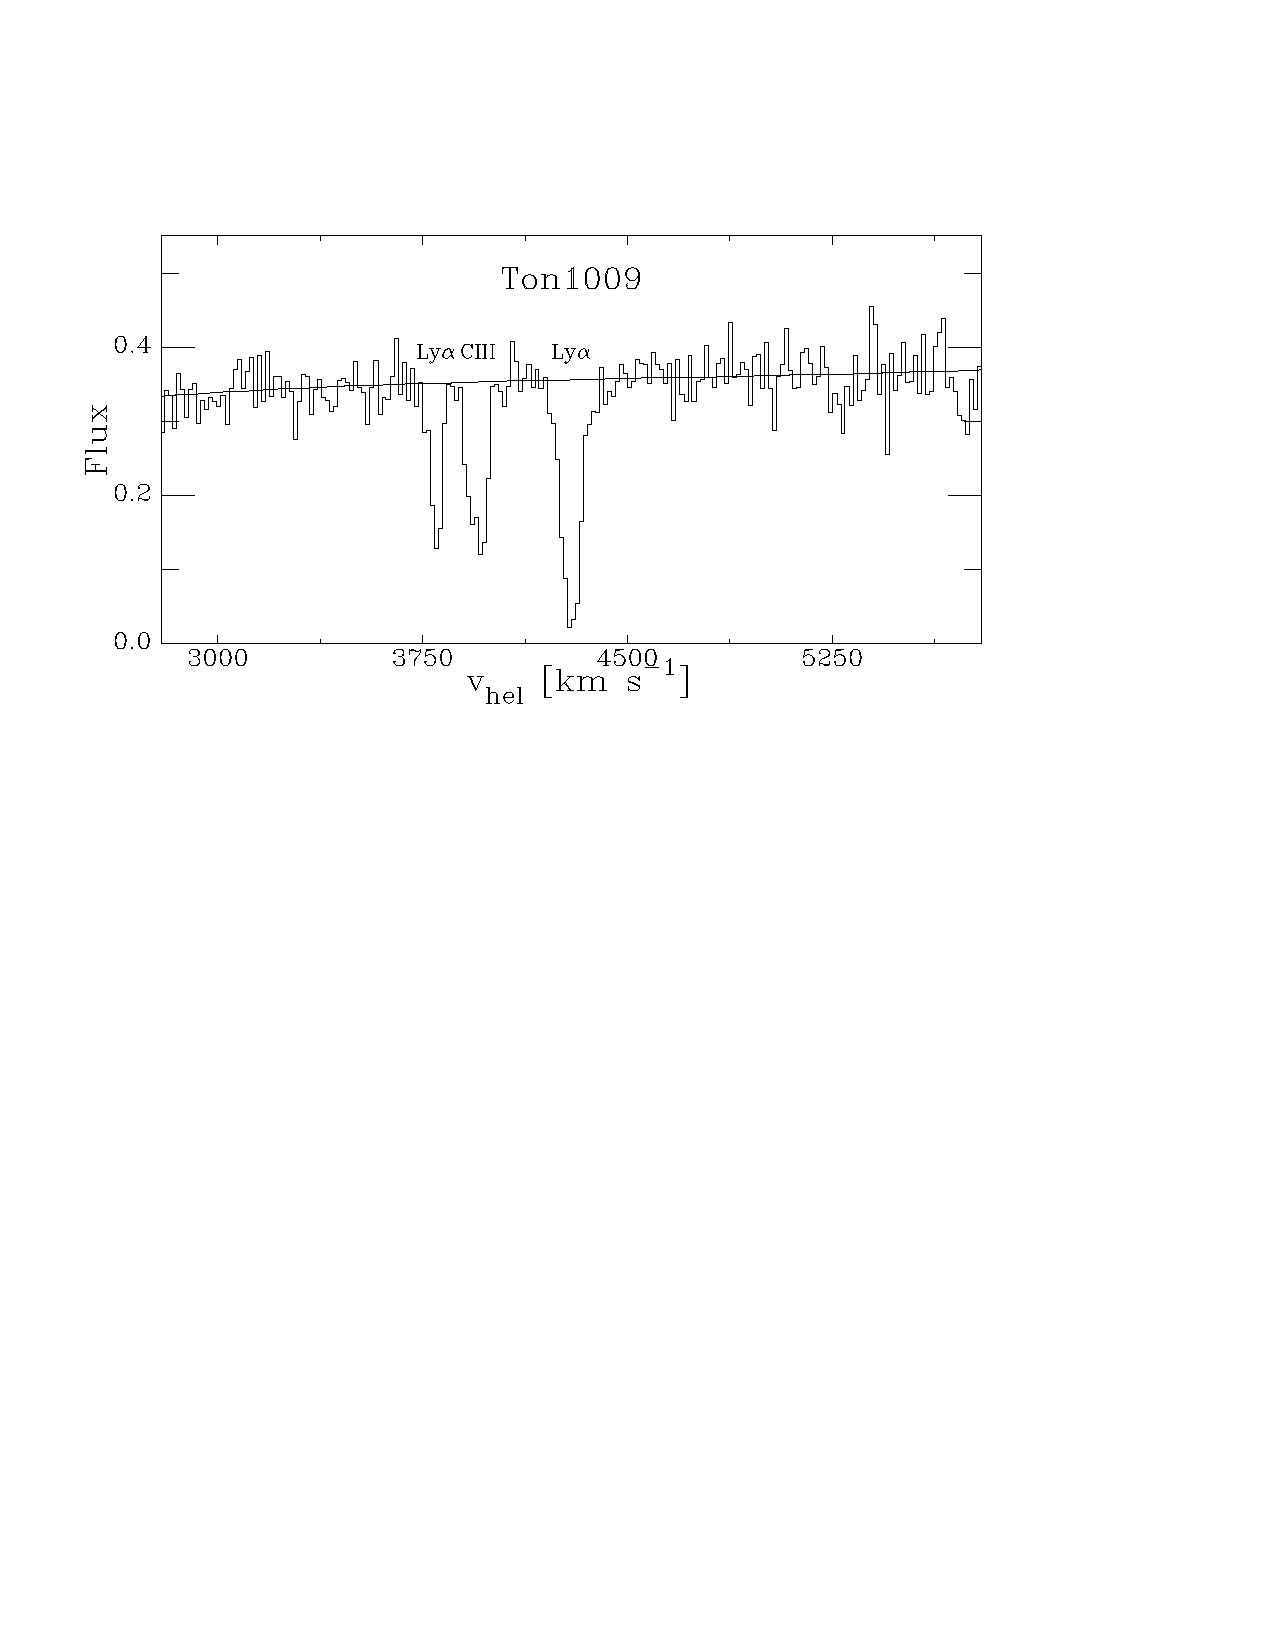
\includegraphics[width=\textwidth]{figTON1009_crop.pdf}
        \caption{}
    \end{subfigure}%
    ~ 
    \begin{subfigure}[t]{0.5\textwidth}
        \centering
        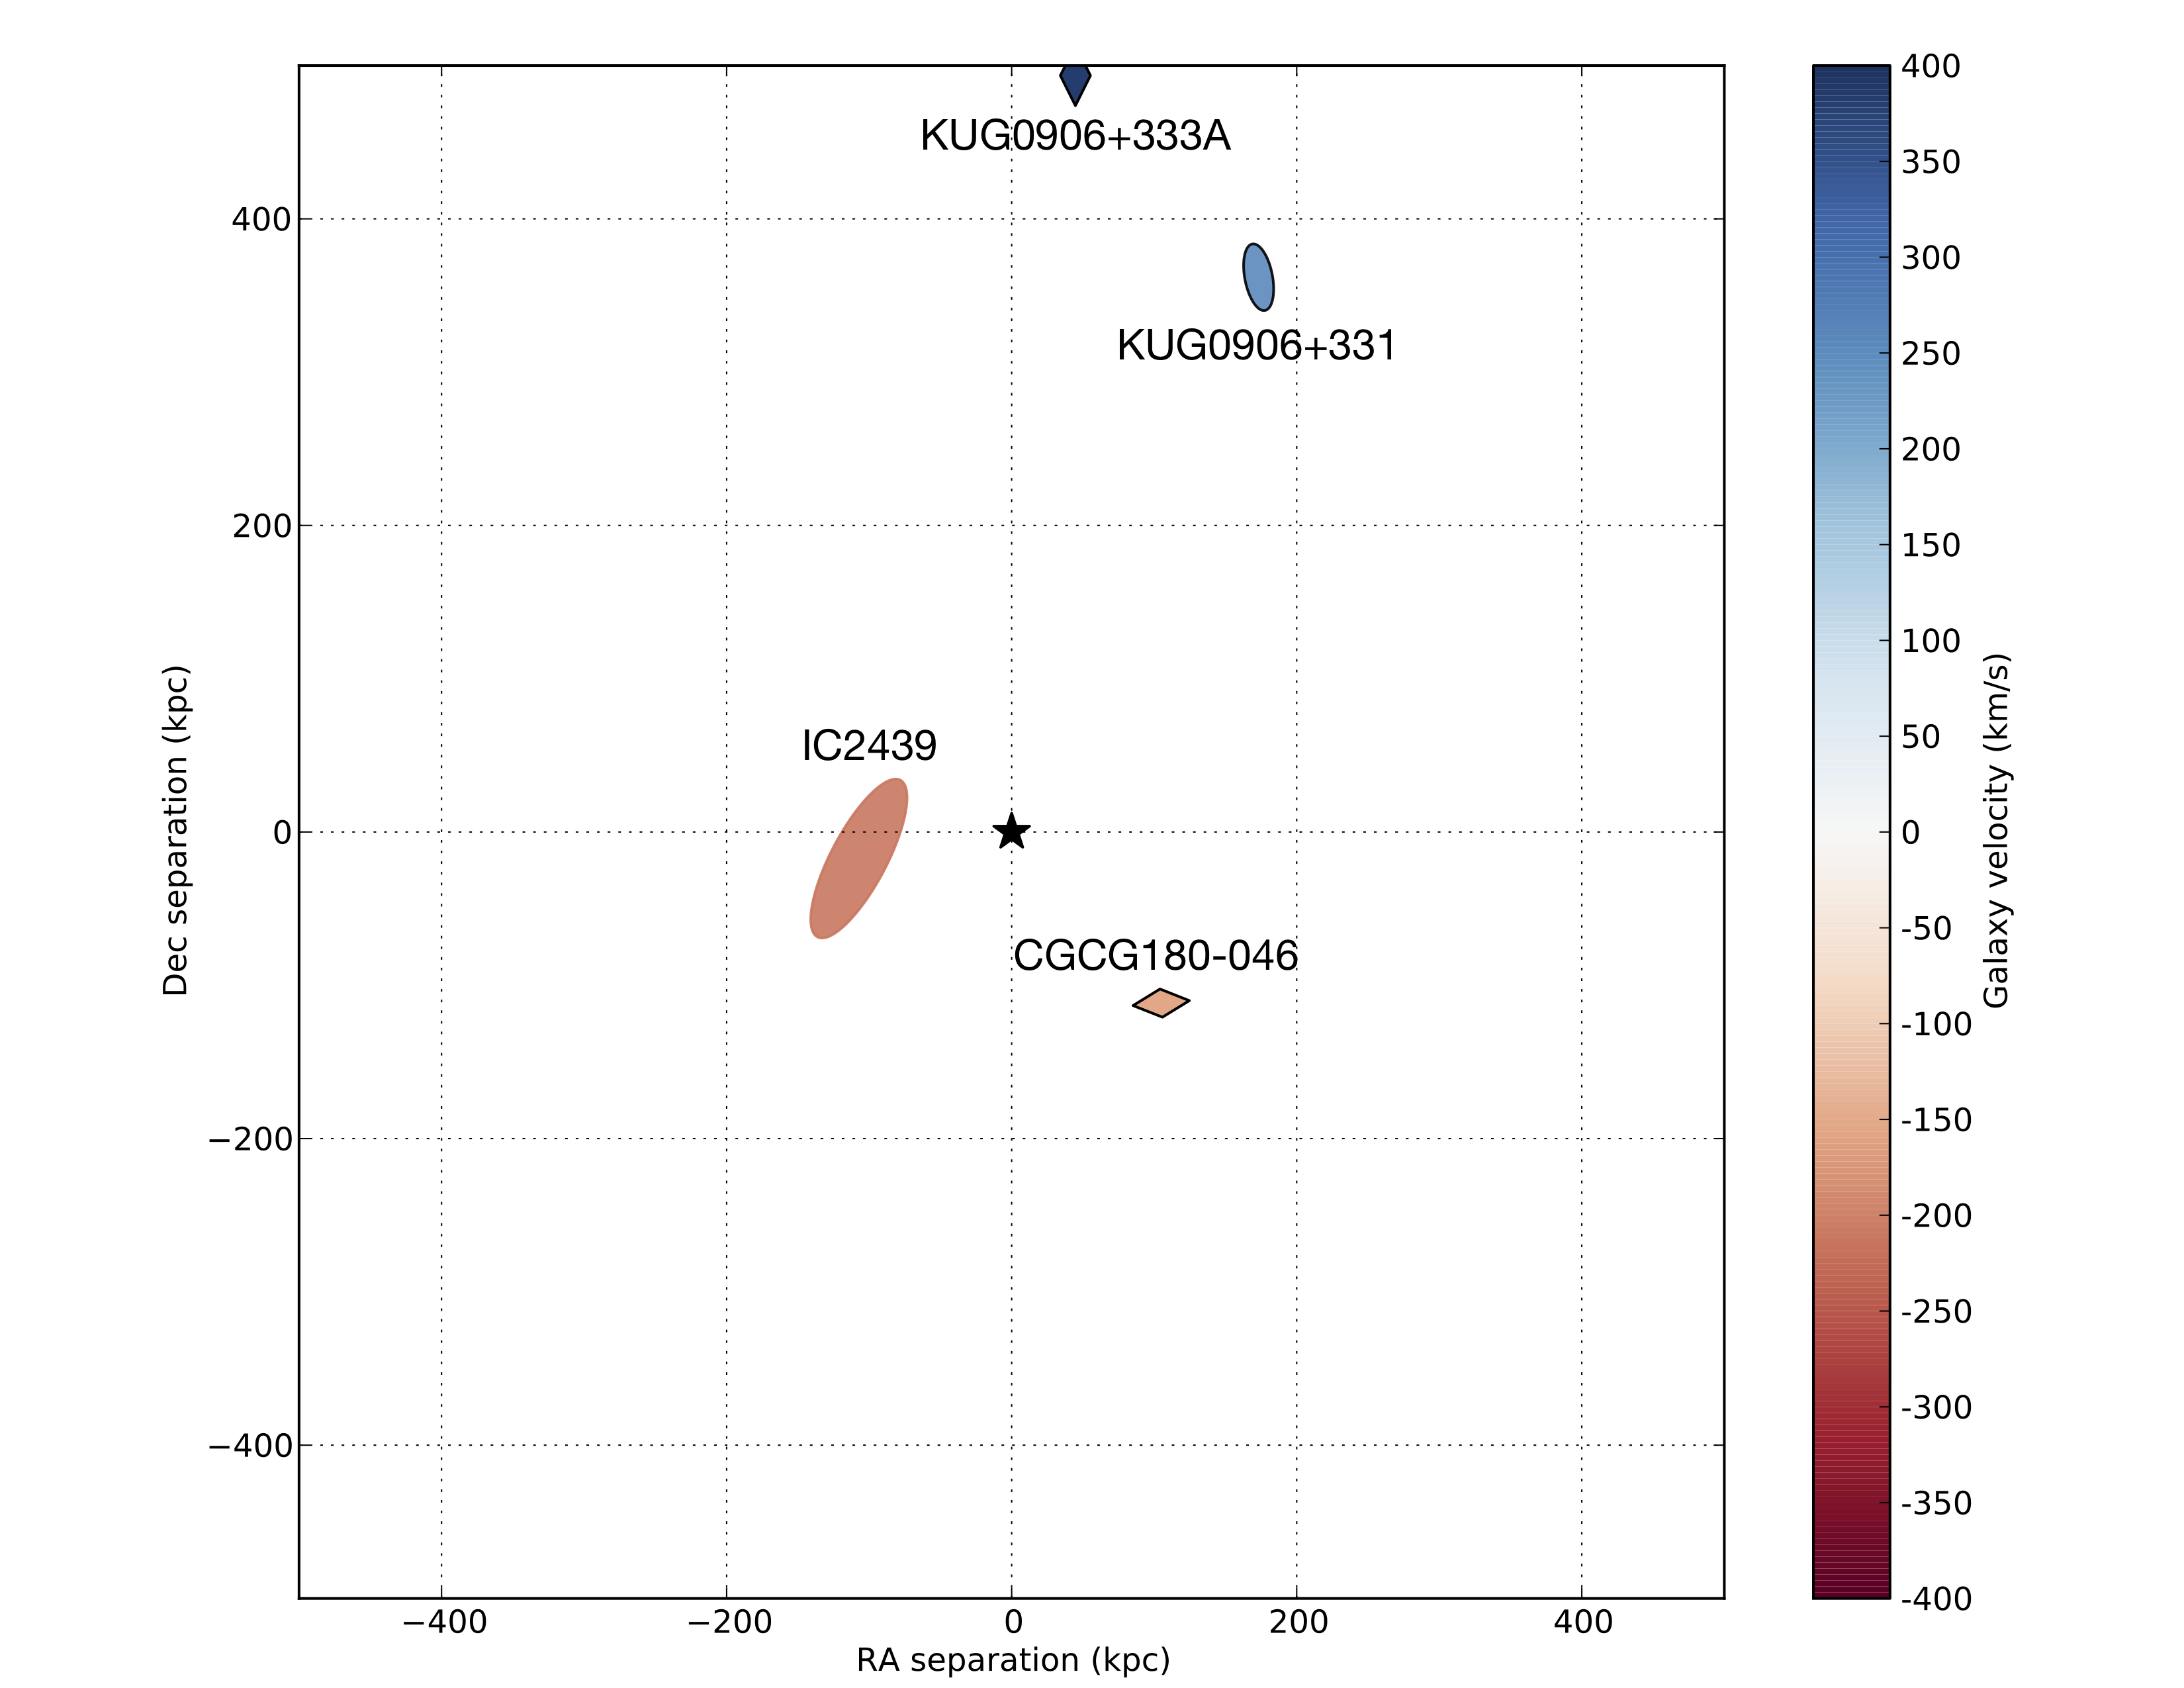
\includegraphics[width=\textwidth]{map_TON1009_4285_crop2_labels.png}
        \caption{}
    \end{subfigure}
  \caption{\small{a) An example Ly$\alpha$ line found in a sightline towards target TON1009 at 4295 km/s. b) A map of \textit{all} galaxies within a 500 kpc impact parameter target TON1009 sightline and with velocity ($cz$) within 400 km/s of absorption detected at 4295 km/s (central black star). The galaxy IC2439 ($v=4494$ km/s, inclination = $71^{\circ}$) can be unambiguously paired with the Ly$\alpha$ absorption feature at $v=4295$ km/s following our selection criteria ($\mathcal{L}_{IC2439} = 0.45$, many times larger than all other nearby galaxies).}}
  \vspace{-10pt}
%    \caption{Caption place holder}
\end{figure}





\noindent \textbf{\underline{3. Incompleteness}}\\

%Other studies supplement archival galaxy data with new observations, but then the search radius is usually limited to a $<10'$ field of view. For example, Mathes et al. (2014) use imaging from the WFPC2 camera on HST, but their impact parameter limit is 300 kpc, close to the commonly accepted boundary between CGM and IGM gas (based on virial radii and/or escape velocity arguments, e.g., see Stocke et al. 2013 and Mathes et al. 2014). 

\textbf{Nearby Galaxy Dataset:} Most CGM studies suffer form limitations due to inhomogeneity and incompleteness in the galaxy data (e.g. at the average redshift of the sample of Werk et al. (2014), $\langle z \rangle \sim 0.2$, the galaxy sample is only complete to $\sim L^{\**}$). To correct for this, we are limiting our study to the redshift range $400$ $\leq$ $cz$ $\leq$ $10,000$ km/s, where available galaxy data is complete to $\sim0.2 L^{\**}$ at $10,000$ km/s, and progressively better towards lower redshifts. We have created a nearby galaxy catalog to aid in our analysis by mining the NASA Extragalactic Database (NED), collecting redshifts, diameters, redshift-independent-distances, morphologies, inclinations, position angles, photometry, and more for each galaxy, and then normalizing these values beyond the basic work done by NED. This catalog is the most complete, comprehensive and up-to-date nearby galaxy catalog in existence (to be published in 2016), and is key to allowing us to draw direct comparisons between the properties of the absorbers in the CGM and the properties of galaxies on a larger scale then ever before.\\

\noindent \underline{\textbf{4. Summary}}
MORE


%%%%%%%%%%%%%%%%%%%%%%%%%%%%%%%%%%%%%%%%%%%%%%%%%%%%%%%%%%%%%%%%%%%%%%%%%%%
%   2. ANALYSIS PLAN
%       (see Section 9.6 of the Call for Proposals)
%
%
\describearchival       % Do not delete this command.
% Enter your analysis plan here.

\textbf{Line Identifications and Measurements:} The analysis begins with aligning and combining multiple exposures to produce a single, clean spectrum. We will then apply the line identification code, the mechanics of which are relatively simple and robust. First, we manually fit gaussian profiles to all spectral features above $2\sigma$ significance. Second, this list of fits is fed into our algorithm, which produces best guess IDs for each feature based on (CITE??) models of IGM abundance. Finally, we inspect each set fits and make small adjustments as needed. In this way each spectrum is both fit by machine and checked by eye, which minimizes miss-fits and machine artifacts. This will result in a dataset of all absorption lines with ID's, velocities, equivalent widths, linewidths, and column density estimates. \\


\noindent \textbf{Galaxy-Absorber Matching:} Next, we will correlate our galaxy dataset with the newly produced absorber dataset. This will produce matched absorber-galaxy systems, complete with association likelihood estimates. Most CGM studies suffer from limitations due to inhomogeneity and incompleteness in the galaxy data. To draw meaningful conclusions from associations between absorbers and galaxies, one must have knowledge of all the nearby galaxies above a reasonable luminosity limit. For example, at the average redshift of the sample of Werk et al. (2014), $\langle z \rangle \sim 0.2$, available galaxy data is only complete to $\sim L^{\**}$ (approximately Milky Way luminosity). Probing gas both very near to as well as physically far from a galaxy is essential to developing a full understanding of the galaxy-IGM interface. This is most easily done in the nearby universe, where the galaxy sample is highly complete to low luminosities. Additionally, by limiting the redshift of our sample, we can include large angular and physical impact parameters, which allows for a wider search for associated QSO sightlines.

\noindent \textbf{New Nearby Galaxy Catalog:} To create a nearby galaxy sample, we have made extensive use of the NASA Extragalactic Database (NED), compiling a table of all pertinent galaxy information in the redshift range $400$ $\leq$ $cz$ $\leq$ $10,000$ km/s. We have collected the redshift, diameter, redshift-independent-distance, inclination, photometry, and more for each galaxy. NED makes an effort to homogenize these data, but we go further by normalizing all measurements of inclination, position angle, and diameter to 2MASS $K$-band values. 2MASS values were chosen as it is an all-sky survey, and measurements are available for the majority of galaxies. Additionally, we calculate best-estimate B-band magnitudes and $L^{\**}$ values from the multitude of disparate photometry values included in NED. This catalog is complete to $\sim0.2 L^{\**}$ at $10,000$ km/s (and progressively better towards lower redshifts), making it the most complete, comprehensive and up-to-date nearby galaxy catalog in existence (to be published in 2016), and is key to allowing us to draw direct comparisons between the properties of the absorbers in the CGM and the properties of galaxies on a larger scale then ever before.\\


\noindent \textbf{Publication}\\
\indent The final data set will be made available publicly in a machine readable format.


%%%%%%%%%%%%%%%%%%%%%%%%%%%%%%%%%%%%%%%%%%%%%%%%%%%%%%%%%%%%%%%%%%%%%%%%%%%

%   3. MANAGEMENT PLAN
%       (see Section 9.7 of the Call for Proposals)
%
%  Provide a concise, but complete, management plan. This plan will be used
%  by the review panels to assess the likely scale of the proposed research
%  program. Proposers should include a schedule of the work required to
%  achieve the scientific goals of the program, a description of the roles of the
%  PI, CoIs, postdocs, and students who will perform the work, and a plan to
%  disseminate the results to the community.
%
\budgetnarrative       % Do not delete this command. CALLS the Management Plan header in the Style File (IGNORE the command name of budgetnarrative
% Enter your management plan here.

\textbf{Line Identifications and Measurements}\\
\indent Spectra prep and line IDing will be led by Wakker, with additional input by French.

\noindent \textbf{Galaxy Matching}\\
\indent Galaxy matching and final dataset preparation will be led by French.



\end{document}          % End of proposal. Do not delete this line.
                        % Everything after this command is ignored.

